\documentclass[16pts]{report}
\usepackage[utf8]{inputenc}
\usepackage[T1]{fontenc}
\usepackage[francais]{babel}
\usepackage{xcolor}
\usepackage[hyphens]{url}
\usepackage[hidelinks]{hyperref}
\usepackage{amsmath}
\usepackage{graphicx}
\usepackage{geometry}
\usepackage{textcomp}
\hypersetup{hypertexnames=true}
\geometry{hmargin=2.5cm,vmargin=1.5cm}

\usepackage{float} %Option H pour les figures, utile.


%\maketitle
%\clearpage

\begin{document}
\bibliographystyle{unsrt}
\nocite{*}

\chapter{Scénario et maquettes}
\label{cha:Scénario et maquettes}

\section{Scénario A: Configuration par défaut}
\label{sec:Scénario A: Configuration par défaut}

\begin{enumerate}
    \item L'utilisateur lance l'application.
    \begin{figure}[H]
        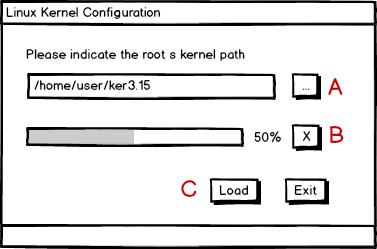
\includegraphics[scale=0.5]{illustrations/maquettes/Maquette_1_first_dialog.png}
        \centering
        \caption{Maquette 1}
        \label{fig:Maq1}
    \end{figure}
    \item L'utilisateur sélectionne le noyau qu'il souhaite configurer
            (Maquette 1 - Élément A).
    \item L'utilisateur valide le noyau qu'il a choisi (Maquette 1 - Élément C).
    \item L'application charge en mémoire les options du noyau et passe à la
            fenêtre suivante lorsque la barre de chargement est pleine (Passe à
            la Maquette 2).
    \begin{figure}[H]
        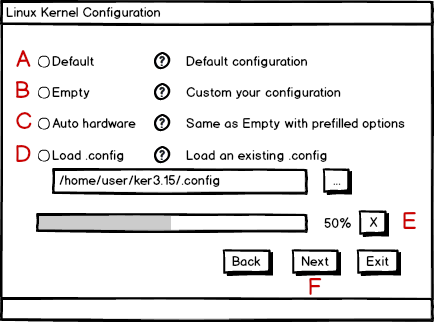
\includegraphics[scale=0.5]{illustrations/maquettes/Maquette_2_choose_dialog.png}
        \centering
        \caption{Maquette 2}
        \label{fig:Maq2}
    \end{figure}
    \item L'utilisateur sélectionne la configuration par défaut (Maquette 2 -
        Élément A).
    \item L’utilisateur clique sur Next (Maquette 2 - Élément F).
    \item L’application sélectionne les options en mémoire pour une
            configuration par défaut. Lorsque la barre de chargement est pleine,
            l’application passe à la fenêtre suivante.
    \begin{figure}[H]
        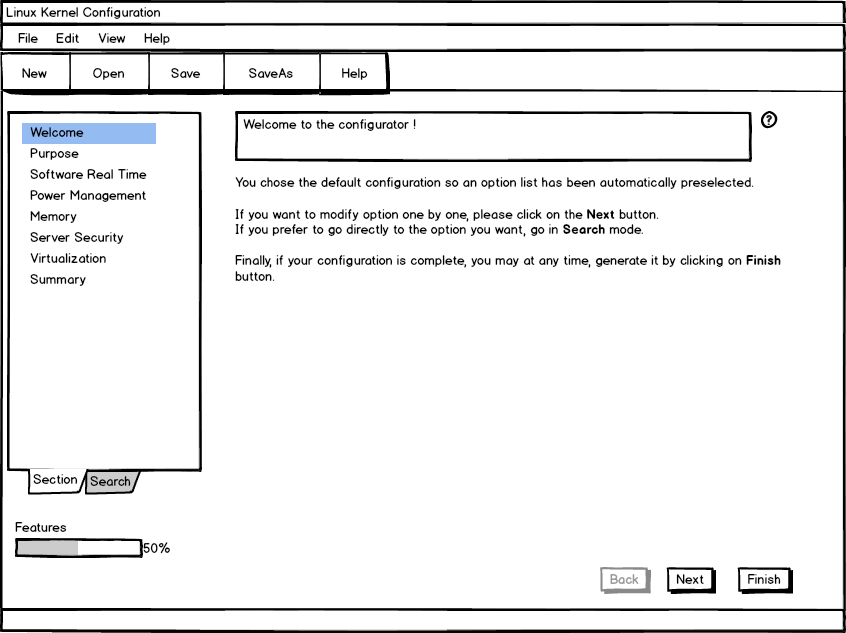
\includegraphics[scale=0.5]{illustrations/maquettes/Maquette_3_MainWindowStart.png}
        \centering
        \caption{Maquette 3}
        \label{fig:Maq3}
    \end{figure}
    \item L’utilisateur valide les options pré-sélectionnées en cliquant sur
        Finish (Maquette 3).
    \item L’application génère le fichier “.config”.
    \item L’utilisateur quitte l’application.
\end{enumerate}

\section{Scénario B: Configuration avancée, modifications, conflits}
\label{sec:Scénario B: Configuration avancée, modifications, conflits}

\begin{enumerate}
    \item Reprendre le scénario A jusqu’à l’étape 4.
    \item L’utilisateur sélectionne la configuration vierge / empty  (Maquette
        2 - Élément B).
    \item L’utilisateur clique sur Next (Maquette 2 - Élément F).
    \item L’application passe à la fenêtre suivante (Passe à la Maquette 3).
    \item L’utilisateur clique sur “next” et l’application passe sur la
        première option (Passe à la Maquette 4).
    \begin{figure}[H]
        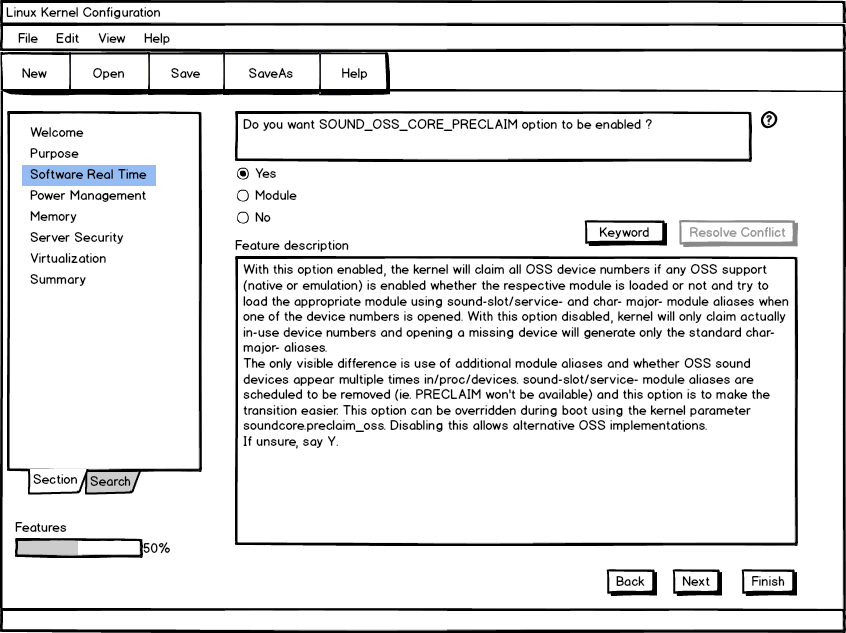
\includegraphics[scale=0.5]{illustrations/maquettes/Maquette_4_MainWindowSection.png}
        \centering
        \caption{Maquette 4}
        \label{fig:Maq4}
    \end{figure}
    \item L’utilisateur clique sur “next” (Maquette 4), ce qui valide le choix
        précédent (l’option est à “yes” par défaut) et passe à l’option suivante.
    \item L’application précise qu’il y a un conflit (l’option est à “yes” par
        défaut) et n’autorise pas l'utilisateur à cliquer sur “next” (Maquette 5).
    \begin{figure}[H]
        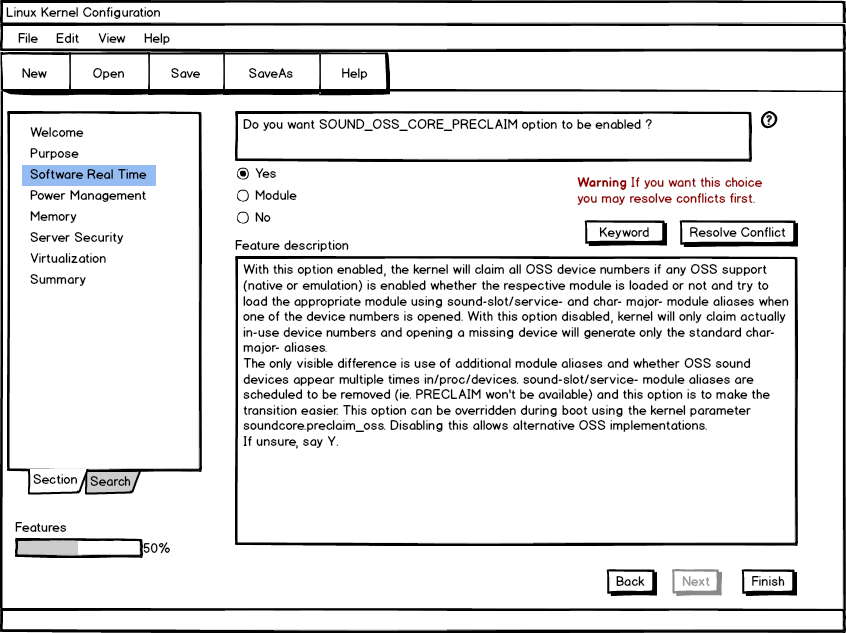
\includegraphics[scale=0.5]{illustrations/maquettes/Maquette_5_MainWindowSectionConflict.png}
        \centering
        \caption{Maquette 5}
        \label{fig:Maq5}
    \end{figure}
    \item L’utilisateur clique sur “resolve conflict” (Maquette 5).
    \item L’application ouvre une fenêtre de résolution des conflits (Maquette
        6) et affiche toutes les options en conflit.
    \begin{figure}[H]
        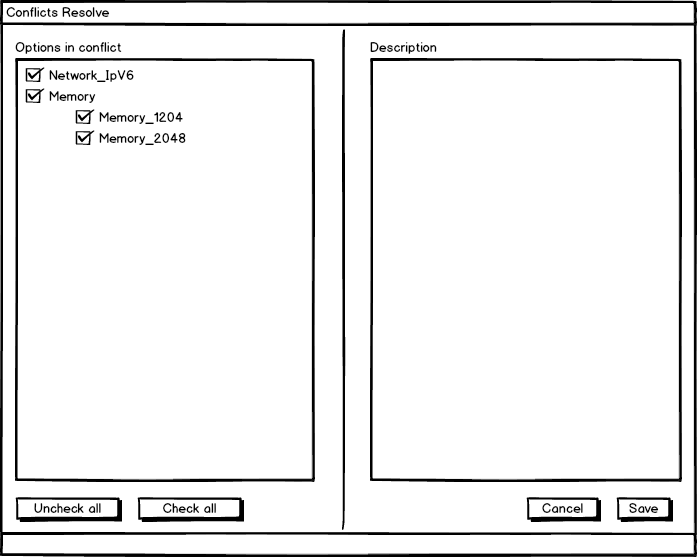
\includegraphics[scale=0.5]{illustrations/maquettes/Maquette_6_resolve_dialog.png}
        \centering
        \caption{Maquette 6}
        \label{fig:Maq6}
    \end{figure}
    \item L’utilisateur clique sur “uncheck all” et valide son choix en cliquant
        sur save (Maquette 6).
    \item L’application applique les changements apportés par l’utilisateur et
        revient à la fenêtre principale (Maquette 4).
    \item L’utilisateur peut dorénavant sélectionner l’option qu’il voulait et
        il clique donc sur “next” (Maquette 4).
    \item L’utilisateur valide les options sélectionnées en cliquant sur Finish
        (Maquette 4).
    \item L’application génère le fichier “.config”.
    \item L’utilisateur quitte l’application.
\end{enumerate}

\section{Scénario C: Configuration par détection du matériel, recherche d'options}
\label{sec:Scénario C: Configuration par détection du matériel, recherche d'options}

\begin{enumerate}
    \item Reprendre le scénario A jusqu’à l’étape 4.
    \item L’utilisateur sélectionne la configuration détection du matériel /
        auto hardware (Maquette 2 - Élément C).
    \item L’utilisateur clique sur Next (Maquette 2 - Élément F).
    \item L’application sélectionne les options qui coïncident avec le matériel
        de l’utilisateur. Lorsque la barre de chargement est pleine,
        l’application passe à la fenêtre suivante (Passe à la Maquette 3).
    \item L’utilisateur clique sur Search (Passe à la Maquette 7).
    \begin{figure}[H]
        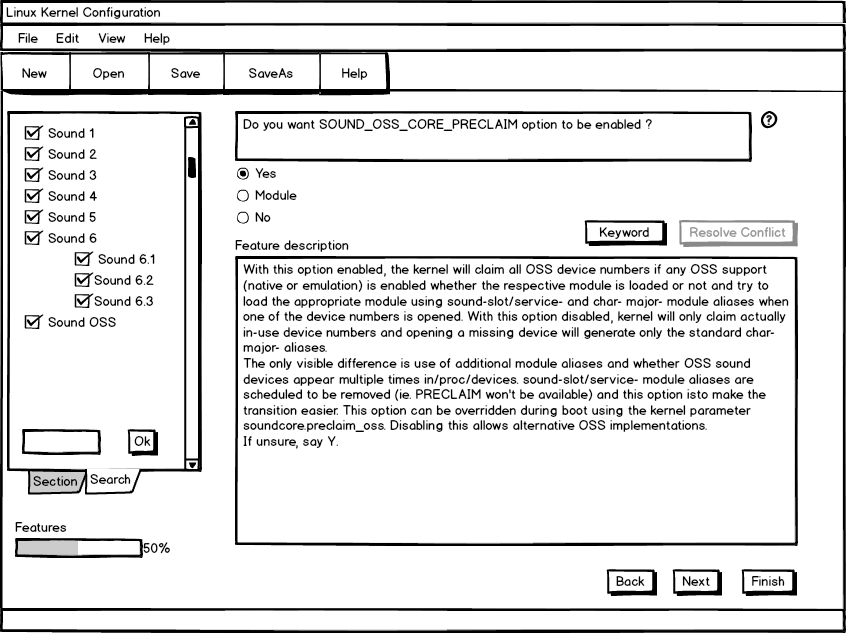
\includegraphics[scale=0.5]{illustrations/maquettes/Maquette_7_MainWindowSearch.png}
        \centering
        \caption{Maquette 7}
        \label{fig:Maq7}
    \end{figure}
    \item L’application affiche une zone de saisie.
    \item L’utilisateur saisit un mot clé pour trouver une option.
    \item L’application affiche les options relatives à ce mot-clé (Maquette 8).
    \begin{figure}[H]
        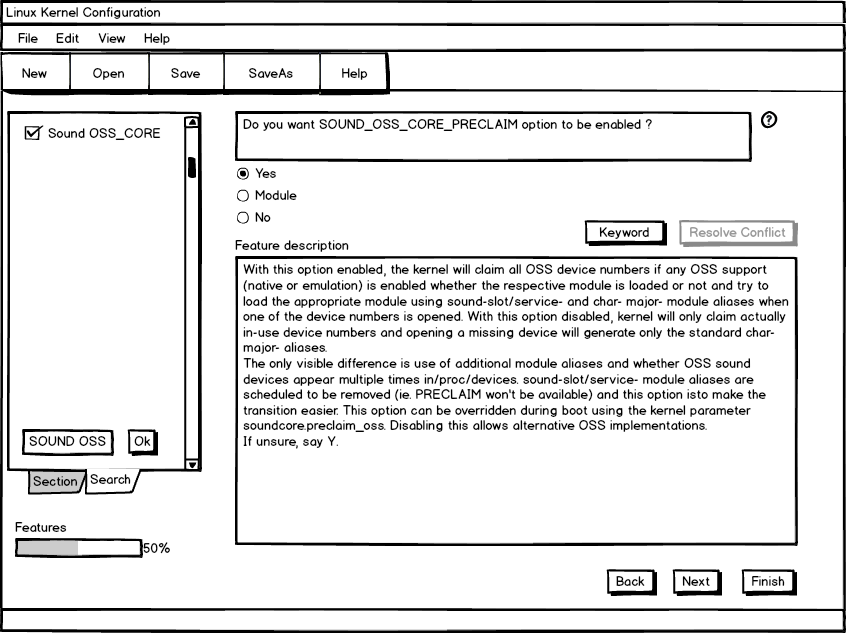
\includegraphics[scale=0.5]{illustrations/maquettes/Maquette_8_MainWindowSearchResult.png}
        \centering
        \caption{Maquette 8}
        \label{fig:Maq8}
    \end{figure}
    \item L’utilisateur peut sélectionner l’option qu’il voulait.
    \item L’utilisateur valide les options sélectionnées en cliquant sur Finish
        (Maquette 8).
    \item L’application génère le fichier “.config”.
    \item L’utilisateur quitte l’application.
\end{enumerate}

\section{Scénario D: Configuration par chargement de fichier de configuration, ajout de mots-clés}
\label{sec:Scénario D: Configuration par chargement de fichier de configuration, ajout de mots-clés}


\begin{enumerate}
    \item Reprendre le scénario A jusqu’à l’étape 4.
    \item L’utilisateur sélectionne la configuration Load .config (Maquette 2 -
        Élément D).
    \item L’application sélectionne les options présentent dans le fichier
        précédemment chargé.
    \item L’utilisateur clique sur Next (Maquette 2 - Élément F).
    \item L’application sélectionne les options présentent dans le fichier
        précédemment chargé. Lorsque la barre de chargement est pleine,
        l’application passe à la fenêtre suivante (Passe à la Maquette 3).
    \item L’utilisateur sélectionne une option et clique sur Keyword (Passe à
        la Maquette 9).
    \begin{figure}[H]
        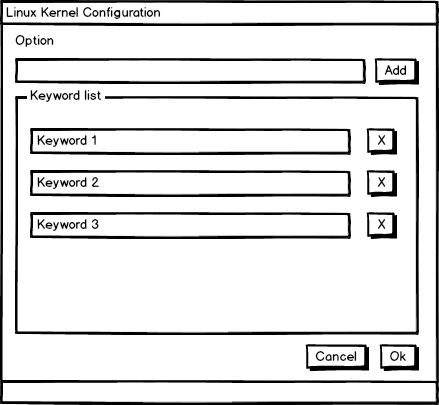
\includegraphics[scale=0.5]{illustrations/maquettes/Maquette_9_keyword_dialog.png}
        \centering
        \caption{Maquette 9}
        \label{fig:Maq9}
    \end{figure}
    \item L’utilisateur saisit le nom d’un mot-clé et valide l’ajout.
    \item L’utilisateur valide les options sélectionnées en cliquant sur Finish.
    \item L’application génère le fichier “.config”.
    \item L’utilisateur quitte l’application.
\end{enumerate}

\chapter{Diagramme des cas d'utilisation}
\label{cha:Diagramme des cas d'utilisation}

\begin{figure}[H]
    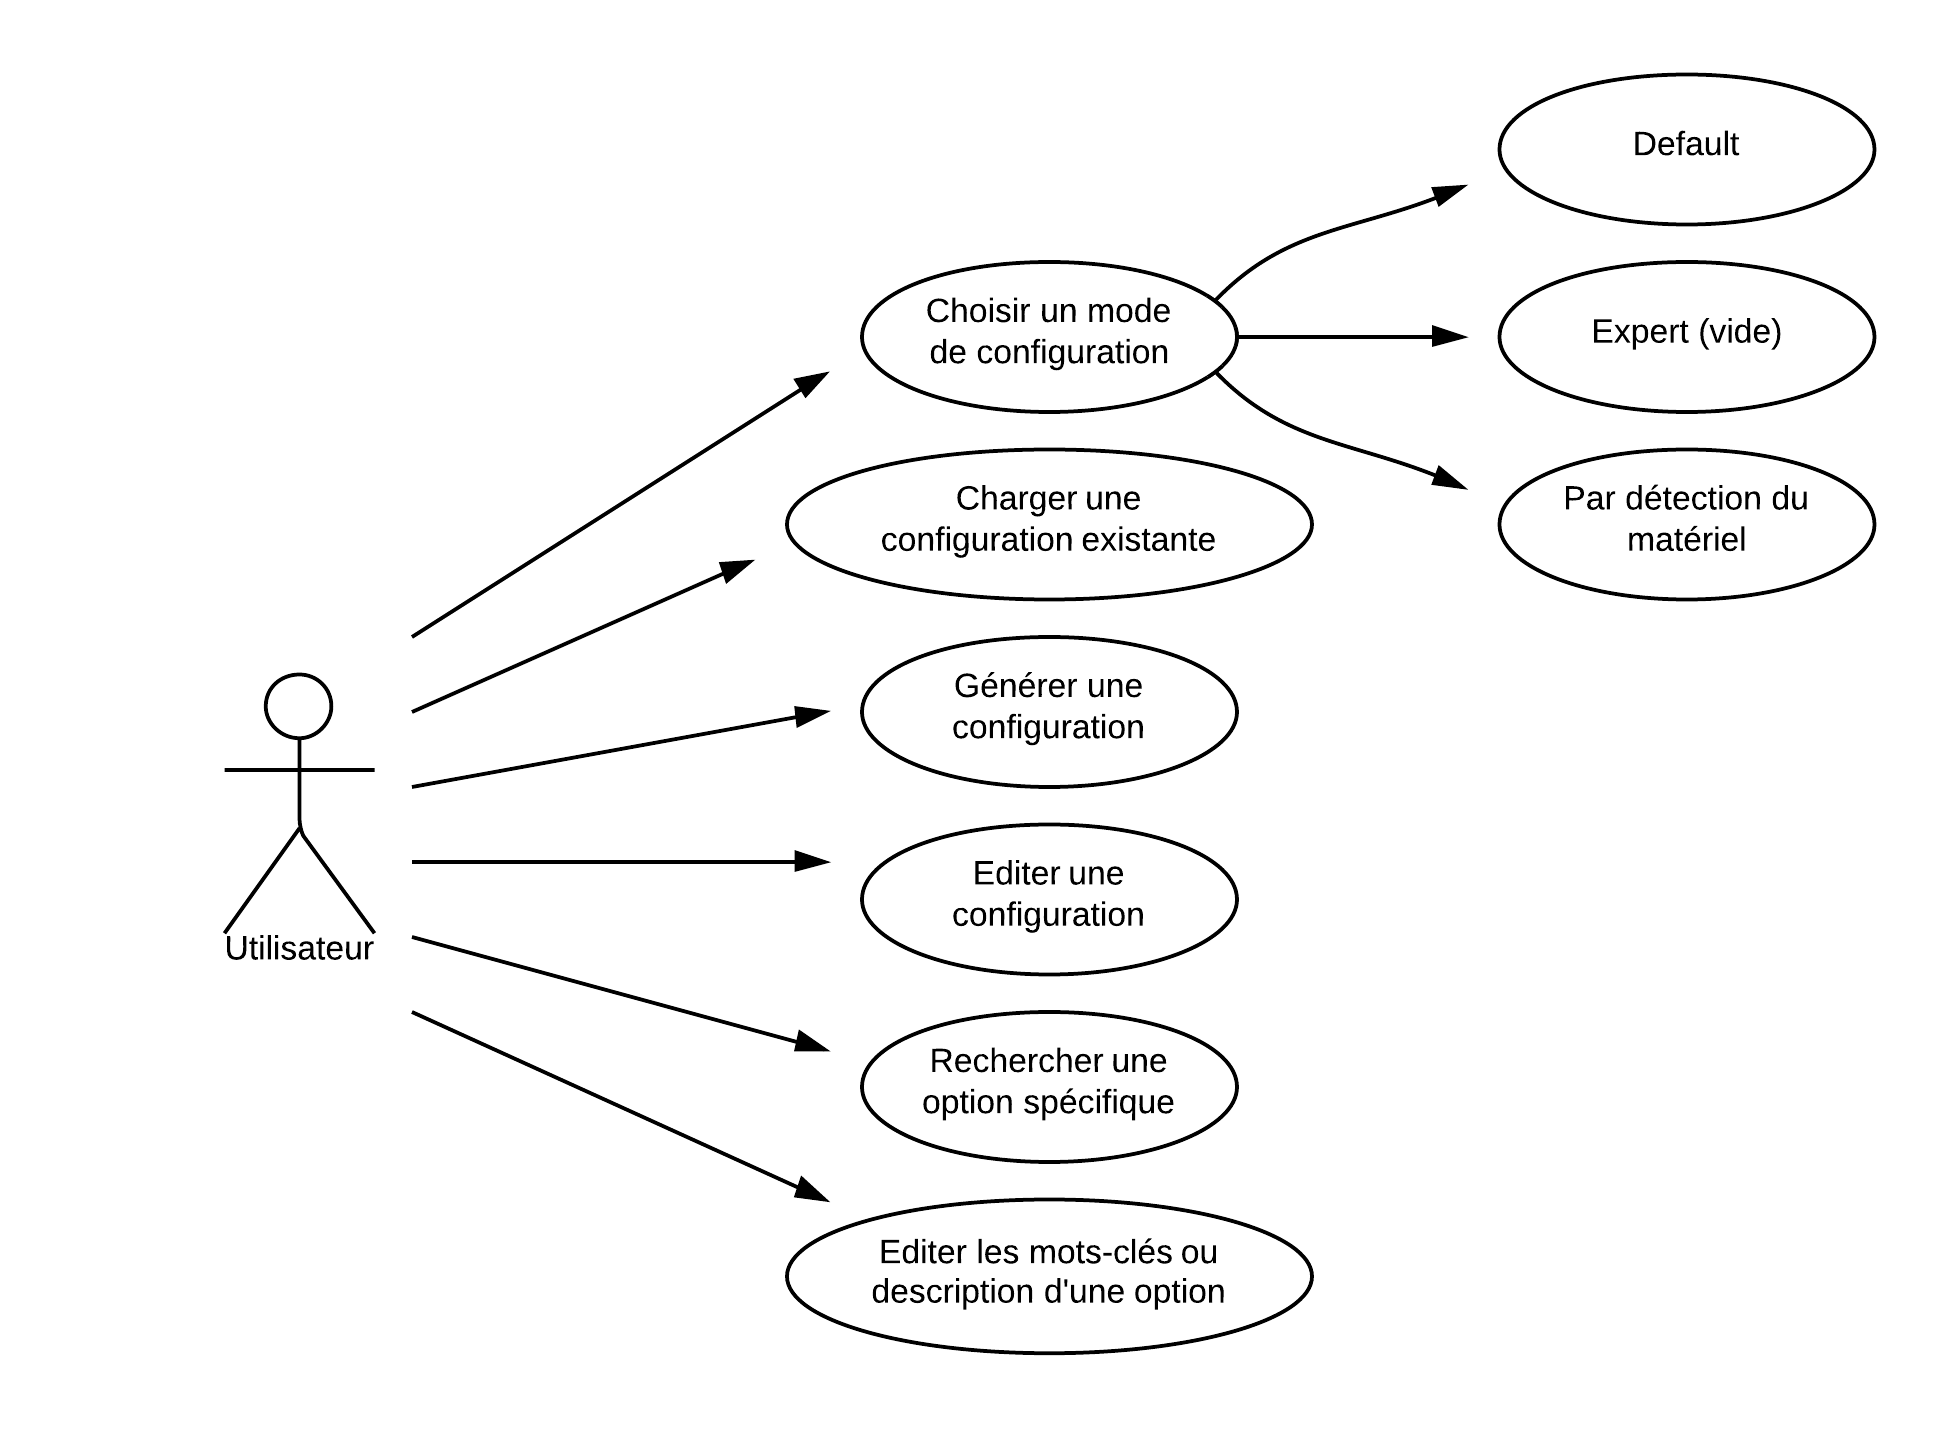
\includegraphics[scale=0.25]{illustrations/diagramme_cas_utilisation.png}
    \centering
    \caption{Diagramme des cas d'utilisation}
    \label{fig:DCU}
\end{figure}

\chapter{Besoins fonctionnels et tests}
\label{cha:Besoins fonctionnels et tests}

\section{Détection du matériel}
\label{sec:Détection du matériel}
\subsection{Besoin}
\label{sub:Besoin}

Il faut qu’un utilisateur puisse détecter son matériel afin de pouvoir
avoir une liste d’options sélectionnées plus précise/adaptée qu’une
configuration par défaut. Un utilisateur désirant un noyau minimal est
confronté aux soucis qui sont de trouver la correspondance entre son matériel et
les options proposées.

Il existe des outils Linux permettant de récupérer la liste du matériel associé
aux bus PCI et USB de la machine hôte.  N’ayant pas trouvé d’outil Linux
permettant de récupérer directement le ou les modules noyau utilisés sur une
entrée, l’étude du contenu des répertoires “/dev /sys” et “/proc” sera
nécessaire afin d’acquérir de plus amples informations.

Afin de rendre la correspondance des modules du noyau Linux au matériel plus
pertinente et fiable, l’idée serait de récupérer des logs d’exécution du scan
du matériel afin de peupler de manière volontaire une base de données
communautaire.

\subsection{Test}
\label{sub:Test}

Si l’utilisateur précise qu’il réalise une configuration pour la machine
courante, l’application devra l’alerter quand celui-ci cherchera à activer une
option incompatible avec son matériel. Par exemple, si sa machine a un
processeur 32-bits et que l’utilisateur sélectionne l’option pour un processeur
64-bits, l’application devra l’avertir que la configuration ne sera pas adaptée
à sa machine. Des tests similaires pourront être proposés pour de nombreuses
options liées au matériel.


\section{Gestion des conflits}
\label{sec:Gestion des conflits}
\subsection{Besoin}
\label{sub:Besoin}

L’application doit pouvoir “gérer les conflits et les dépendances” entre les
options de configuration. Grâce au fichier kconfig, l’application pourra, pour
chaque option de configuration, connaître ses dépendances et les options avec
lesquelles elle rentre en conflit. De ce fait, chaque fois que l’utilisateur
sélectionne ou désélectionne une option de configuration, des tests sont
effectués par l'application pour savoir si cette option entre en conflit avec
une autre (si elle est cochée) ou génère une erreur de dépendance (si elle est
décochée).

\subsection{Test}
\label{sub:Test}

La sélection d’une option doit signaler à l’utilisateur l’éventuelle présence
d’un conflit. Il doit également lui être proposé de pouvoir le résoudre. Or,
trouver une solution est un problème NP-complet. En effet, à chaque nouvelle
option il faut vérifier les dépendances de toutes les options précédemment
cochées. Il est possible qu’une option précédente exclût la nouvelle option.
Toutes les options du fichier de configuration en cours d’édition doivent être
vérifiées, ce qui est impossible en un temps polynomial.

Il faudrait vérifier que les conflits présents dans les fichiers Kconfig du
noyau soient bien affichés dans notre outil.


\section{Recherche}
\label{sec:Recherche}
\subsection{Besoin}
\label{sub:Besoin}

L’utilisateur doit pouvoir effectuer une recherche sur le nom, la description
et les mots-clés relatifs à une option lors de la configuration du noyau. La
fonction de recherche ne posera pas de véritable problème technique.
L’utilisateur pourra faire défiler les lignes contenant les occurrences du
terme recherché.

\subsection{Test}
\label{sub:Test}

Vérifier que la fonction de recherche retourne bien les résultats attendus. Par
exemple, nous pourrons ouvrir un des outils existants (xconfig, gconfig) et
réaliser une recherche. On effectuera la même recherche sur notre outil et on
pourra vérifier si les résultats sont similaires (ce test ne sera valable que
pour les titres des options).


\section{Génération et chargement du fichier .config}
\label{sec:Génération et chargement du fichier .config}
\subsection{Besoin}
\label{sub:Besoin}

L’utilisateur doit pouvoir sauvegarder où il le souhaite le fichier de
configuration généré par l’application. Un message avertira l’utilisateur de la
présence de conflits ou d’erreurs de dépendance avant que la génération ne soit
faite.

La reprise d’un fichier .config doit permettre à un utilisateur de charger une
configuration existante. Le chargement d’un fichier .config corrompu provoquera
une erreur, et les options inconnues (s’il y en a) seront simplement ignorées.
Cela impliquera le déclenchement du mécanisme de résolution des conflits.

\subsection{Tests}
\label{sub:Tests}

Vérifier que le fichier de configuration (.config) soit compatible avec
l’application lors de son chargement. Ce dernier doit respecter le format
d’origine, afin que nous puissions récupérer les informations qui nous sont
utiles.

Vérifier que le fichier de configuration que nous générons via notre outil
peut être chargé (toujours via notre outil) et qu’il contienne les mêmes
données. Pour réaliser ce test, on générera à nouveau un fichier de
configuration et on pourra vérifier après ces trois étapes (génération >
chargement > génération) si les informations sont restées les mêmes. Cela
montrera que la génération et le chargement fonctionnent correctement.


\section{Mots-clés et description d'une option}
\label{sec:Mots-clés et description d'une option}

Un utilisateur doit pouvoir sélectionner une option et y ajouter un mot-clé.
Par exemple, il peut spécifier qu’une option possède le mot-clé “Network”. Il
pourra également supprimer et modifier les mots-clés existants. De la même
façon, l’utilisateur pourra éditer la description d’une option.

\section{Plateforme de partage communautaire}
\label{sec:Plateforme de partage communautaire}

S’il le souhaite, l’utilisateur peut envoyer sur la plateforme de partage, la
correspondance entre le matériel et le module capable de le faire fonctionner,
enrichissant ainsi la base de données de la plateforme.  De la même façon, lors
de la détection du matériel, l’application pourra trouver les modules à activer
(dans le fichier .config) grâce à cette plateforme. Celle-ci servira également
à stocker les “descriptions” et les “mots-clés” des options.


\chapter{Besoins non fonctionnels}
\label{cha:Besoins non fonctionnels}
\section{Facilité d'utilisation}
\label{sec:Facilité d'utilisation}

Notre projet consiste à améliorer l’utilisation des fonctionnalités de base des
outils existants, en les rendant plus accessibles. On a pu constater que le
système de recherche des options n’est pas simple à prendre en main et que la
gestion des conflits pouvait être améliorée.

Nous avons décidé d’améliorer la recherche en scrutant au sein des descriptions
des options en plus de leurs noms. De plus, nous affichons les options pouvant
créer des conflits, ainsi que des informations sur leur provenance.

\section{Profil des utilisateurs}
\label{sec:Profil des utilisateurs}

Actuellement, les outils de configuration d’un noyau Linux sont “réservés” aux
personnes averties. Il faut donc que les fonctionnalités recherchées soient
présentes. Ces améliorations permettront de toucher un plus large public, de
débutant à expert.

\section{Portabilité}
\label{sec:Portabilité}

Il y a deux aspects liés à la portabilité. Dans un premier temps, il est
possible que l’environnement dans lequel l’application sera exécutée ne possède
pas de serveur X (interface graphique). Par conséquent, une solution
privilégiant une interface console (comme Ncurse) serait donc intéressante
puisqu’elle conviendrait à la fois à l’utilisation de l’application sur un
serveur et sur un ordinateur personnel (ou même sur tout type de support
supportant un noyau Linux). Cependant, l’application se voulant être tout
public, une interface lancée depuis la console pourrait se montrer un peu
austère pour un utilisateur habitué à une interface graphique plus
“traditionnelle”.  Dans un second temps, l’application pourra être
fonctionnelle sur un système d’exploitation Windows.

\section{Contraintes légales}
\label{sec:Contraintes légales}

Cet outil étant, open source, nous avons choisi d’utiliser la licence GPLv3.
Cela permettra la reprise éventuelle de ce projet dans l’avenir.

\section{Interface web}
\label{sec:Interface web}

L’utilisateur devrait pouvoir réaliser la détection de son matériel à partir
d’une interface web (comme le site : ma-config.com).

\chapter{Priorité des besoins}
\label{cha:Priorité des besoins}

\begin{tabular}{|c|c|}
    \hline
    Besoin & Priorité \\
    \hline
    \hline
    Génération du fichier .config & Haute \\
    \hline
    Gestion des conflits & Haute \\
    \hline
    Chargement d'un fichier .config & Haute \\
    \hline
    Utilisation de l'application sur un bureau & Haute \\
    \hline
    Recherche & Haute \\
    \hline
    Mots-clés et description d'une option & Moyenne \\
    \hline
    Plateforme de partage communautaire & Moyenne \\
    \hline
    Détection du matériel & Moyenne \\
    \hline
    Peuplement de la base pour la détection de matériel & Faible \\
    \hline
    Utilisation de l'application sur un serveur & Faible \\
    \hline
\end{tabular}


\end{document}
